\documentclass[../main.tex]{subfiles}

\begin{document}

\subsection{Overview}

Se desarrolla una aplicación móvil para iOS cuyo objetivo es interpretar el alfabeto de la lengua de signos americana. Permitirá seleccionar videos mediante diferentes métodos de entrada o la cámara del dispositivo, realizará predicciones sobre los datos de entrada y mostrará por pantalla los resultados. La aplicación está desarrollada únicamente para iPhone y ha sido probada con un iPhone 12 Pro. Es posible que funcione en dispositivos de menor potencia pero no está entre los objetivos del proyecto.

Landscape right es la única orientación soportada por el proyecto, además para obtener los mejores resultados, es recomendable que el dispositivo esté sujeto con un trípode para mejorar su estabilidad. La configuración del proyecto se puede ver en la figura \ref{figure18}.

\begin{figure}[h]
\centering 
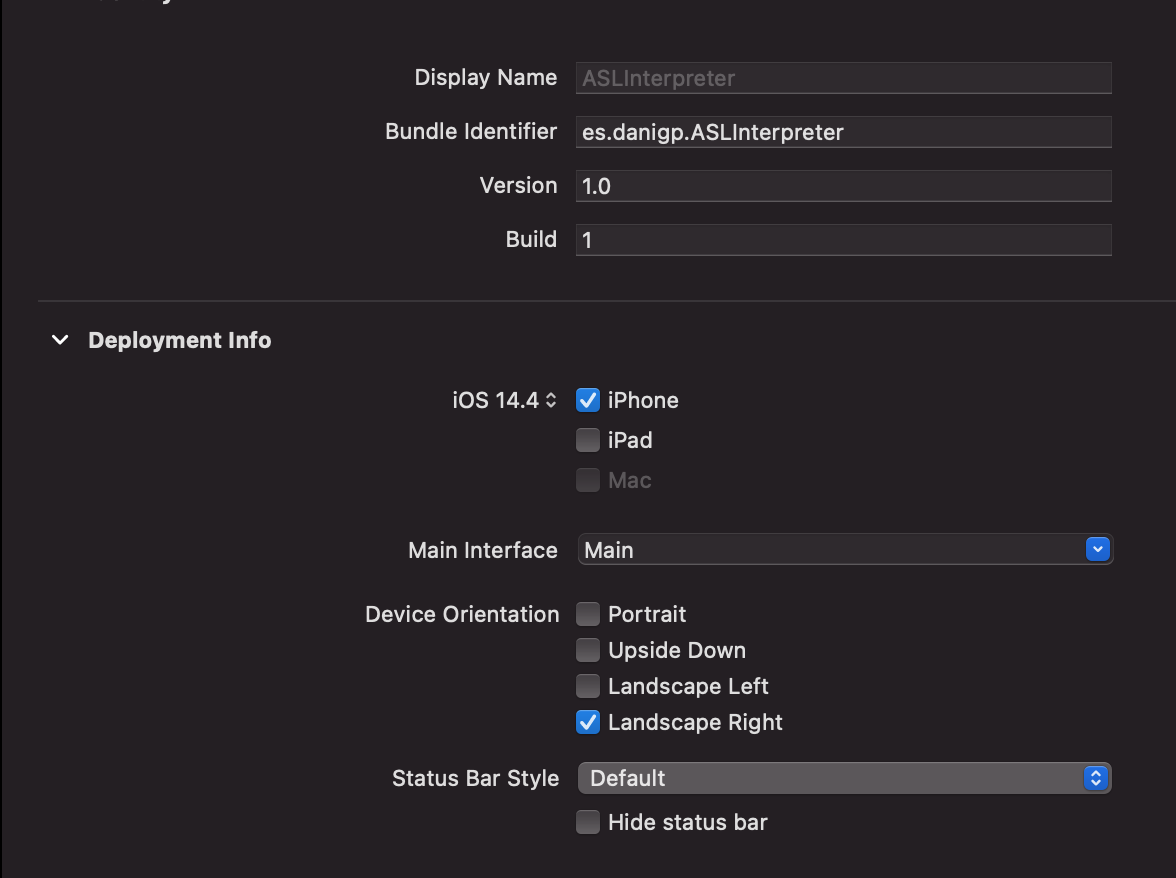
\includegraphics[width=1\textwidth]{images/interpreter/config-project.png}
\caption{Configuración del proyecto en Xcode.}
\label{figure18}
\end{figure}

\subsection{Arquitectura}

La aplicación se desarrolla en Swift 5 y siguiendo la arquitectura Clean Swift Architecture \cite{cleanswift}. Los objetivos de esta arquitectura son los siguientes:

\begin{enumerate}
    \item Disminuir la importancia del controlador: Habitualmente en la arquitectura más comúnmente usada en el desarrollo de aplicaciones para iOS, Model View Controller,  el controlador acaba realizando la mayor parte del trabajo. En esta arquitectura, el controlador pasará a ser parte de la vista y el Interactor será el encargado de realizar la parte lógica de la aplicación, pudiendo utilizar diferentes Workers para ello.
    \item Seguir un flujo de comunicación unidireccional: La comunicación entre los componentes siguen siempre la misma dirección \ref{figure19} 
\end{enumerate}


\begin{figure}
    \centering
    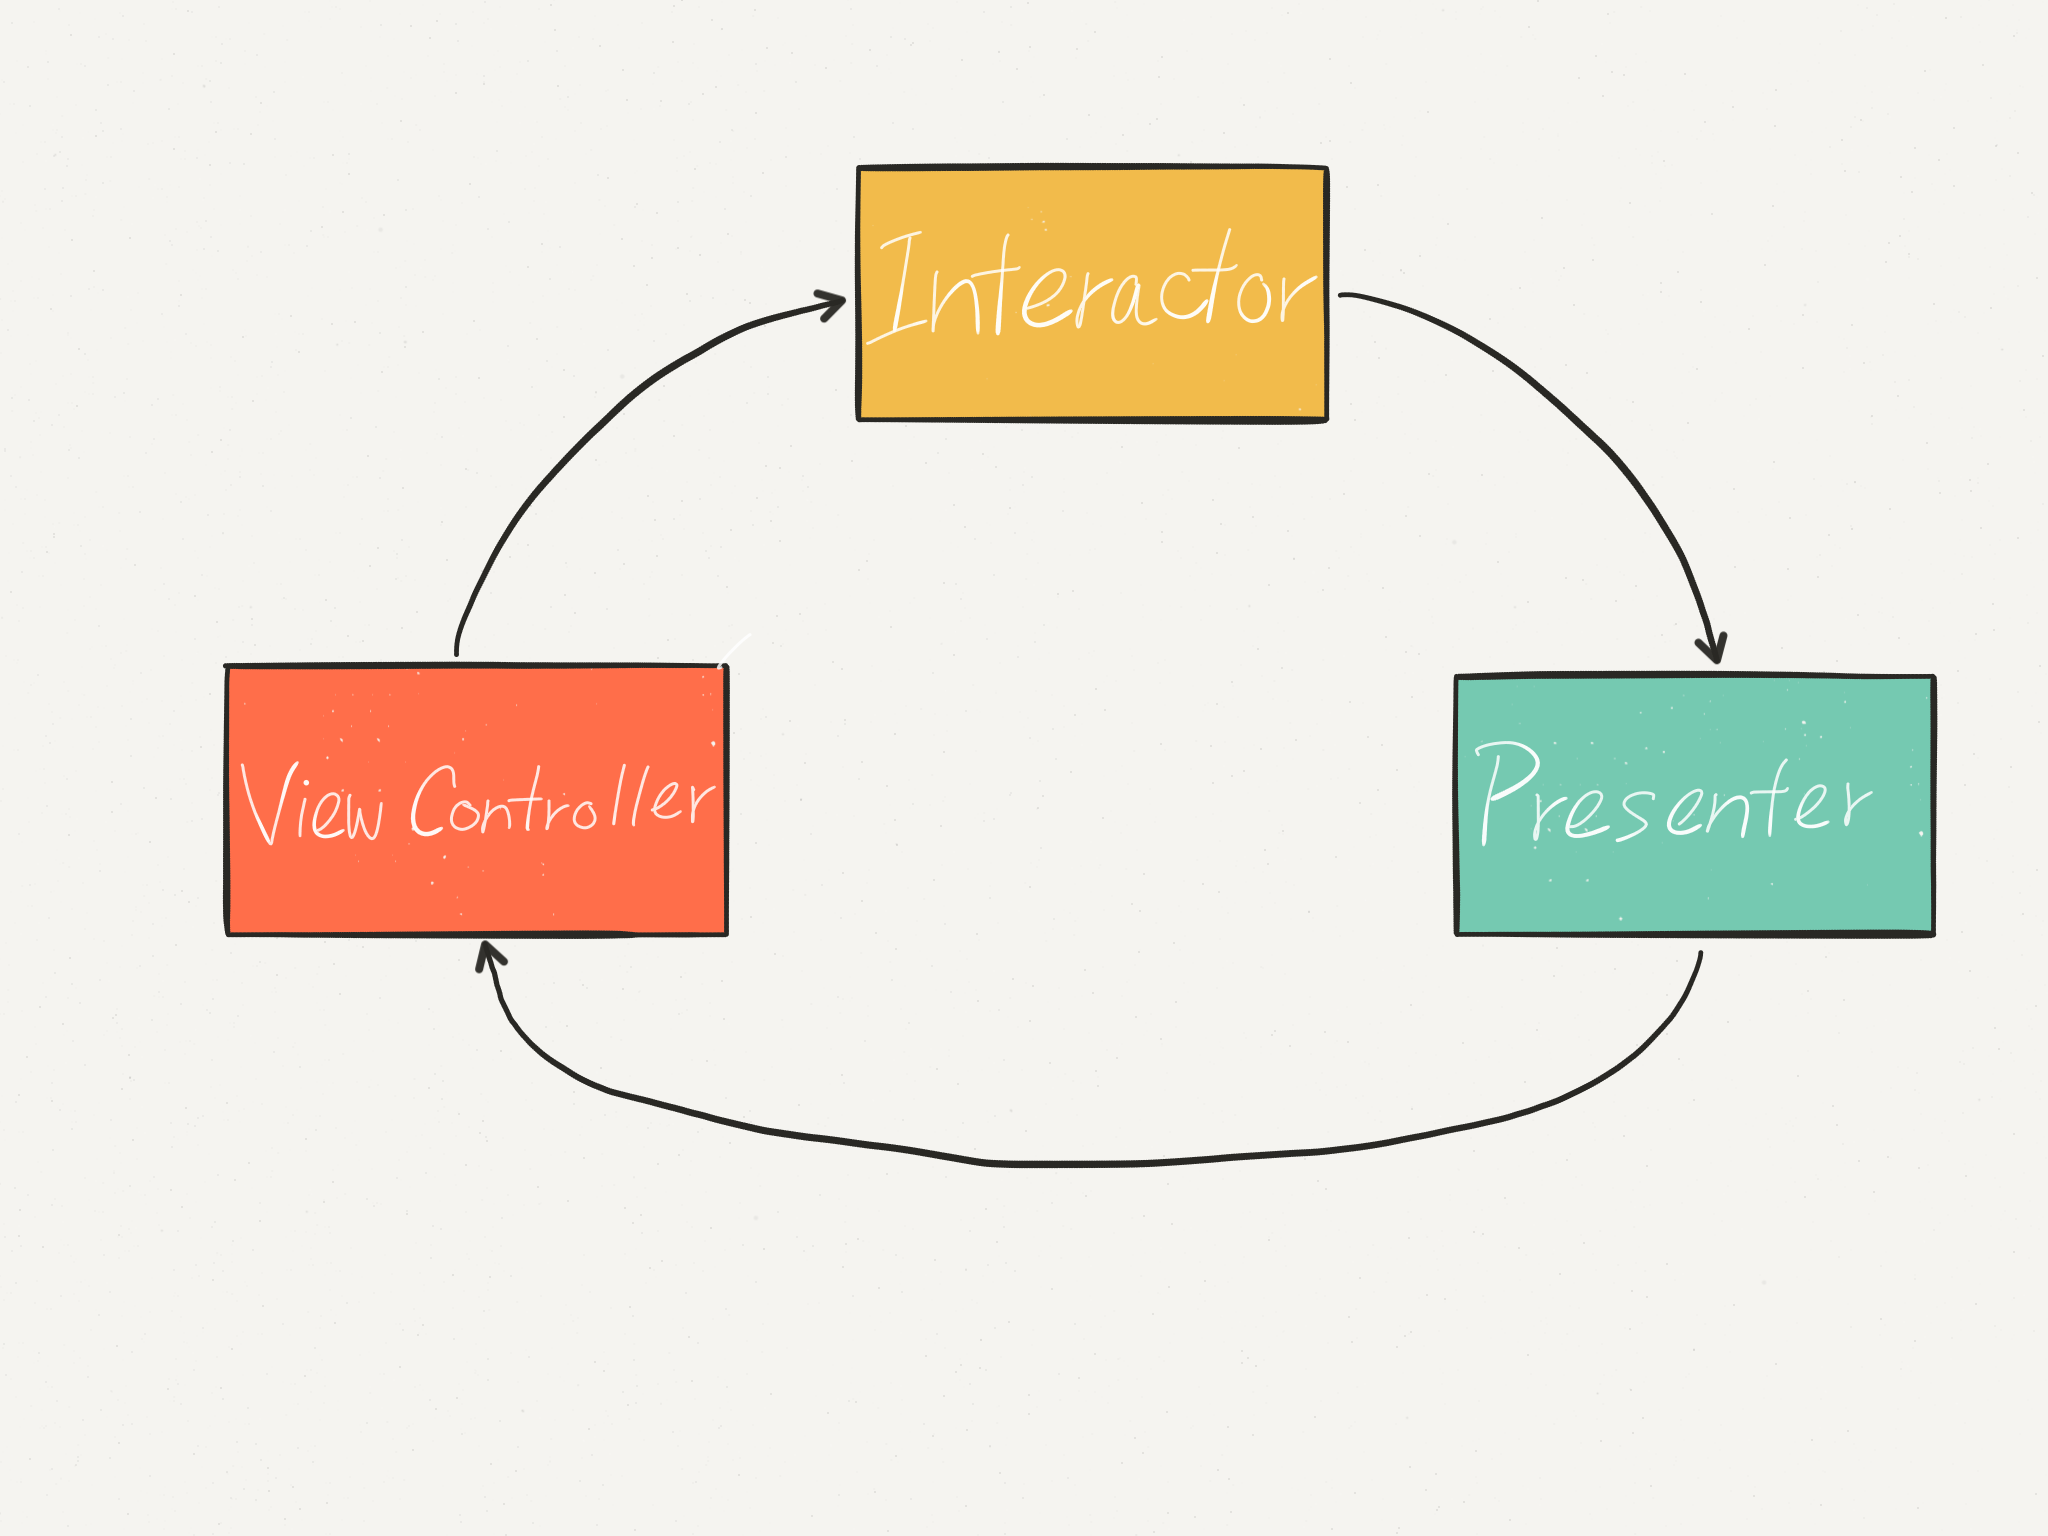
\includegraphics[width=1\textwidth]{images/interpreter/VIP-Cycle.png}
    \caption{\href{http://clean-swift.com/wp-content/uploads/2015/08/VIP-Cycle.png}{Clean Swift Cycle}}
    \label{figure19}
\end{figure}

Siguiendo esta arquitectura, la aplicación cuenta con las siguientes escenas:

\begin{itemize}
    \item Source picker: Encargada de escoger el método de entrada, puede ser tanto la cámara del dispositivo como vídeos. Los videos pueden estar localizados tanto en el propio dispositivo como en iCloud.
    \item Configuración: Permite seleccionar diferentes configuraciones de funcionamiento. Se almacenan de forma persistente para ser usadas entre diferentes ejecuciones.
    \item Overlay: Escena encargada de coordinar los datos de entrada con el intérprete de ASL. Esta escena no es visible pero su función es presentar y coordinar las siguientes escenas.
    \item Cámara: Se encarga de proporcionar un buffer de imágenes para su uso por el intérprete. Obtiene los frames desde la cámara del dispositivo o desde un fichero de video y los transmite al intérprete.
    \item Intérprete: Recibe un buffer de imágenes y realiza predicciones sobre el modelo de Deep Learning. Tras un proceso de refinamiento los resultados se muestran por pantalla. 
\end{itemize}

\subsection{Source Picker}

Es la escena inicial de la aplicación. Permite seleccionar cuál va a ser la fuente de datos. La interfaz se puede ver en la figura \ref{figure20}, y cuenta con las siguientes opciones:

\begin{itemize}
    \item Live Camera: Se selecciona utilizar la cámara del dispositivo. La escena no necesita realizar ninguna acción en este caso.
    \item Library: Permitirá seleccionar un video desde la librería de fotos de iOS. Para ello, se utilizará la clase UIImagePickerViewController que se encarga de mostrar la interfaz de selección de videos y devolver un fichero de video en caso de que sea seleccionado. La interfaz se puede ver en la figura \ref{figure21}
    \item iCloud: Permitirá seleccionar vídeos desde iCloud. Se utiliza la clase UIDocumentPickerViewController que se encarga de mostrar la interfaz de selección de videos y devolver un fichero de video en caso de que sea seleccionado. La interfaz se puede ver en la figura \ref{figure22}
    \item Configuración: Permite dirigirse a la escena de configuración de la aplicación.
\end{itemize}

Si se ha seleccionado una entrada de datos, se dirige a la escena Overlay para su procesamiento.

\begin{figure}[h]
\centering 
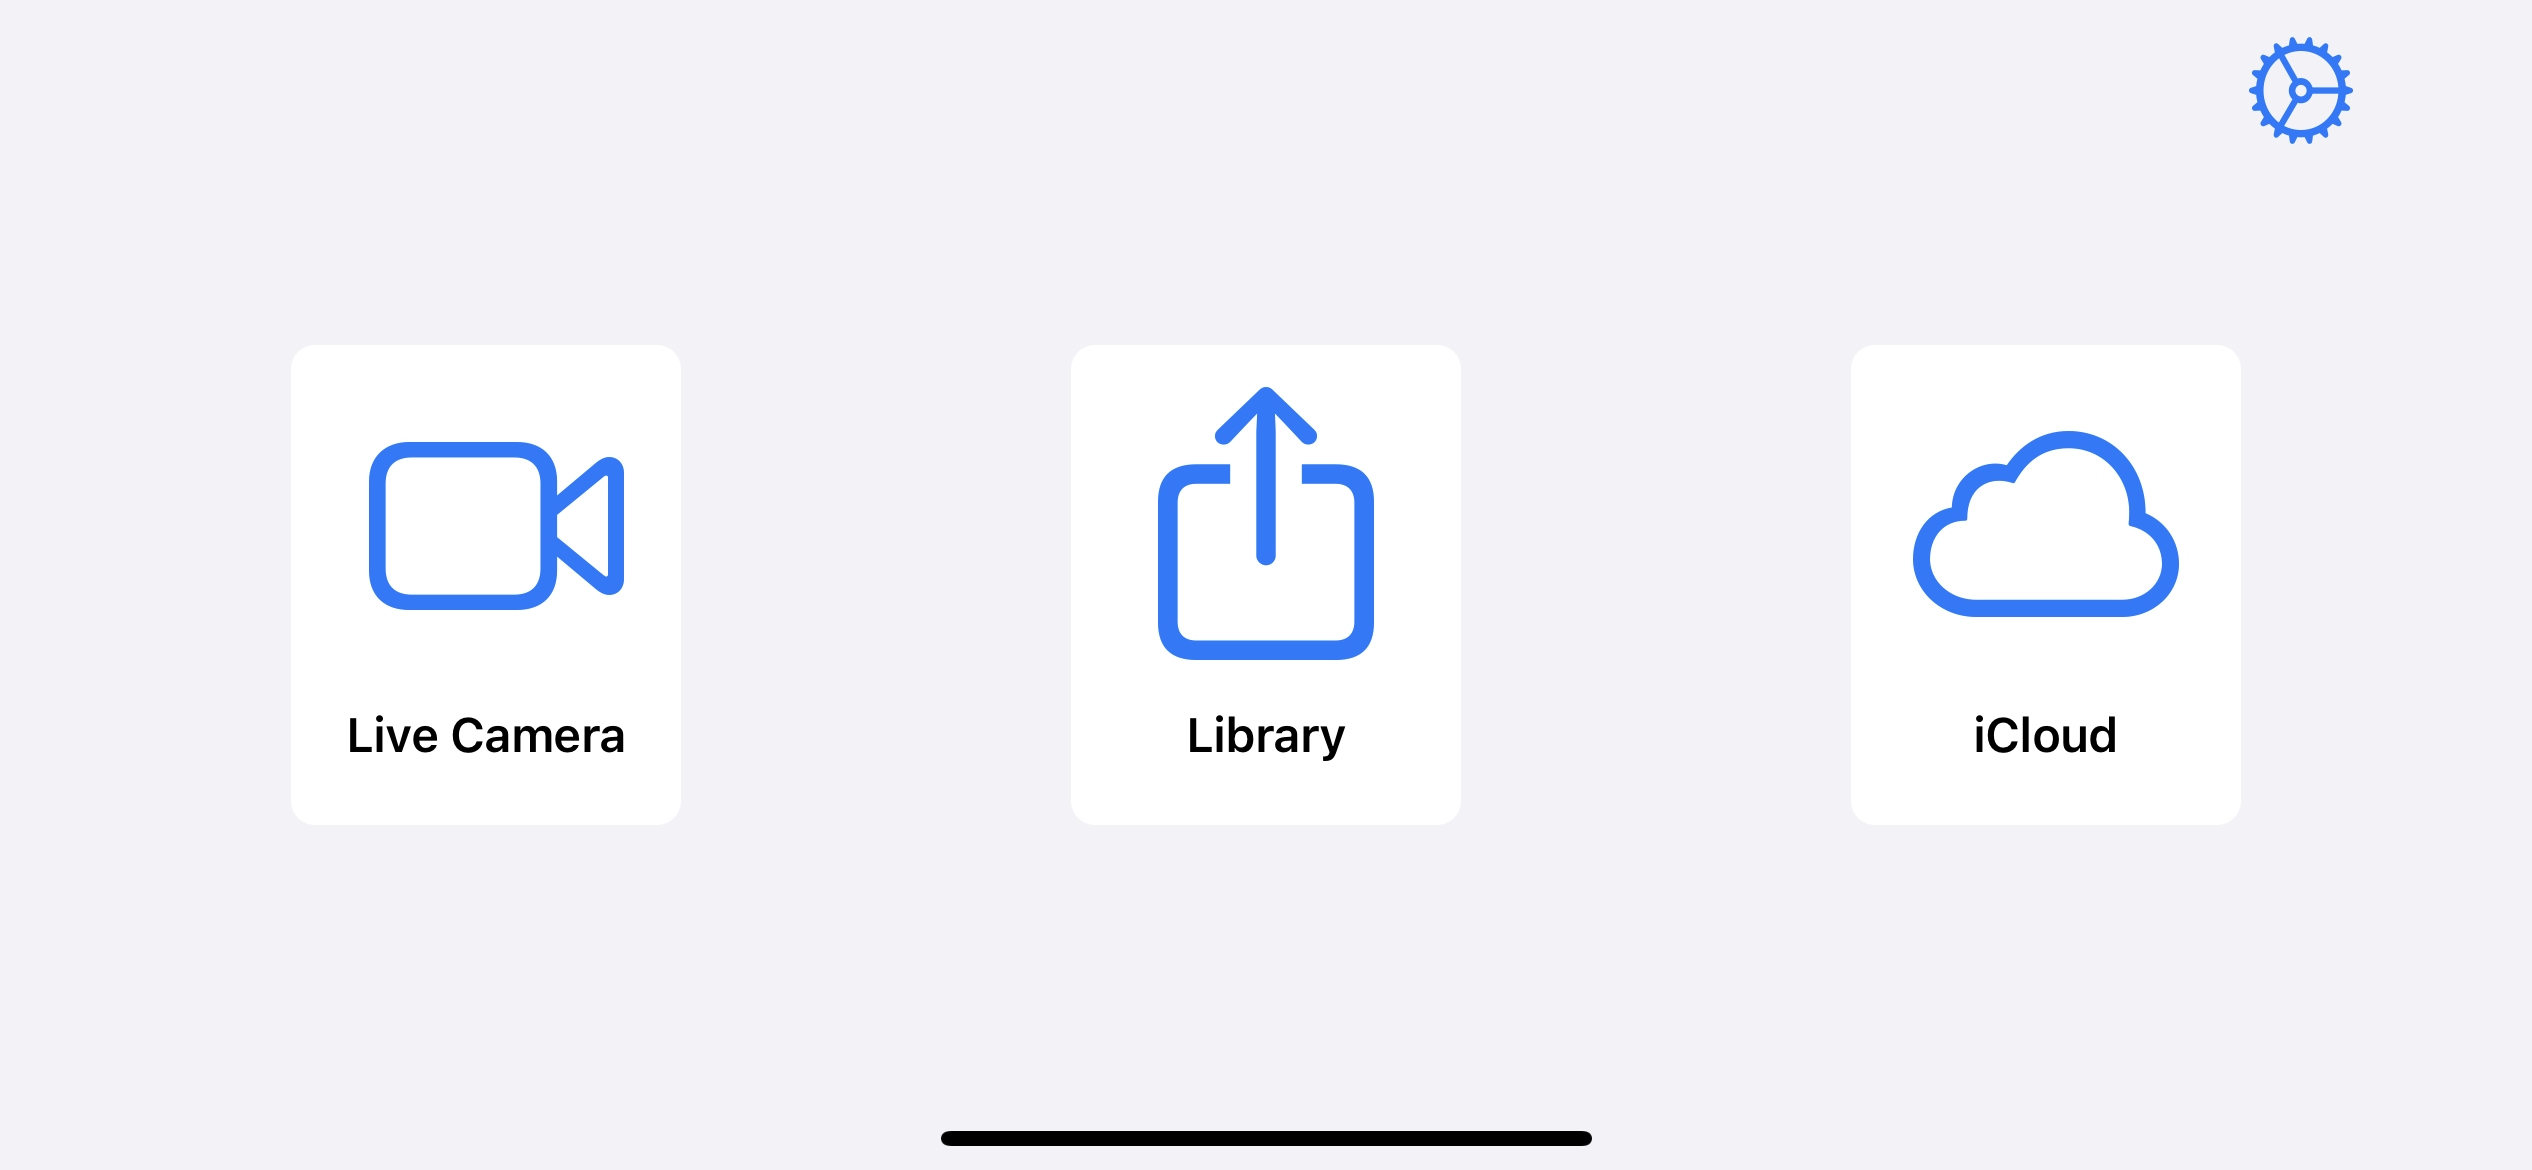
\includegraphics[width=1\textwidth]{images/interpreter/picker.PNG}
\caption{Interfaz de la escena Picker View.}
\label{figure20}
\end{figure}

\begin{figure}[h]
\centering 
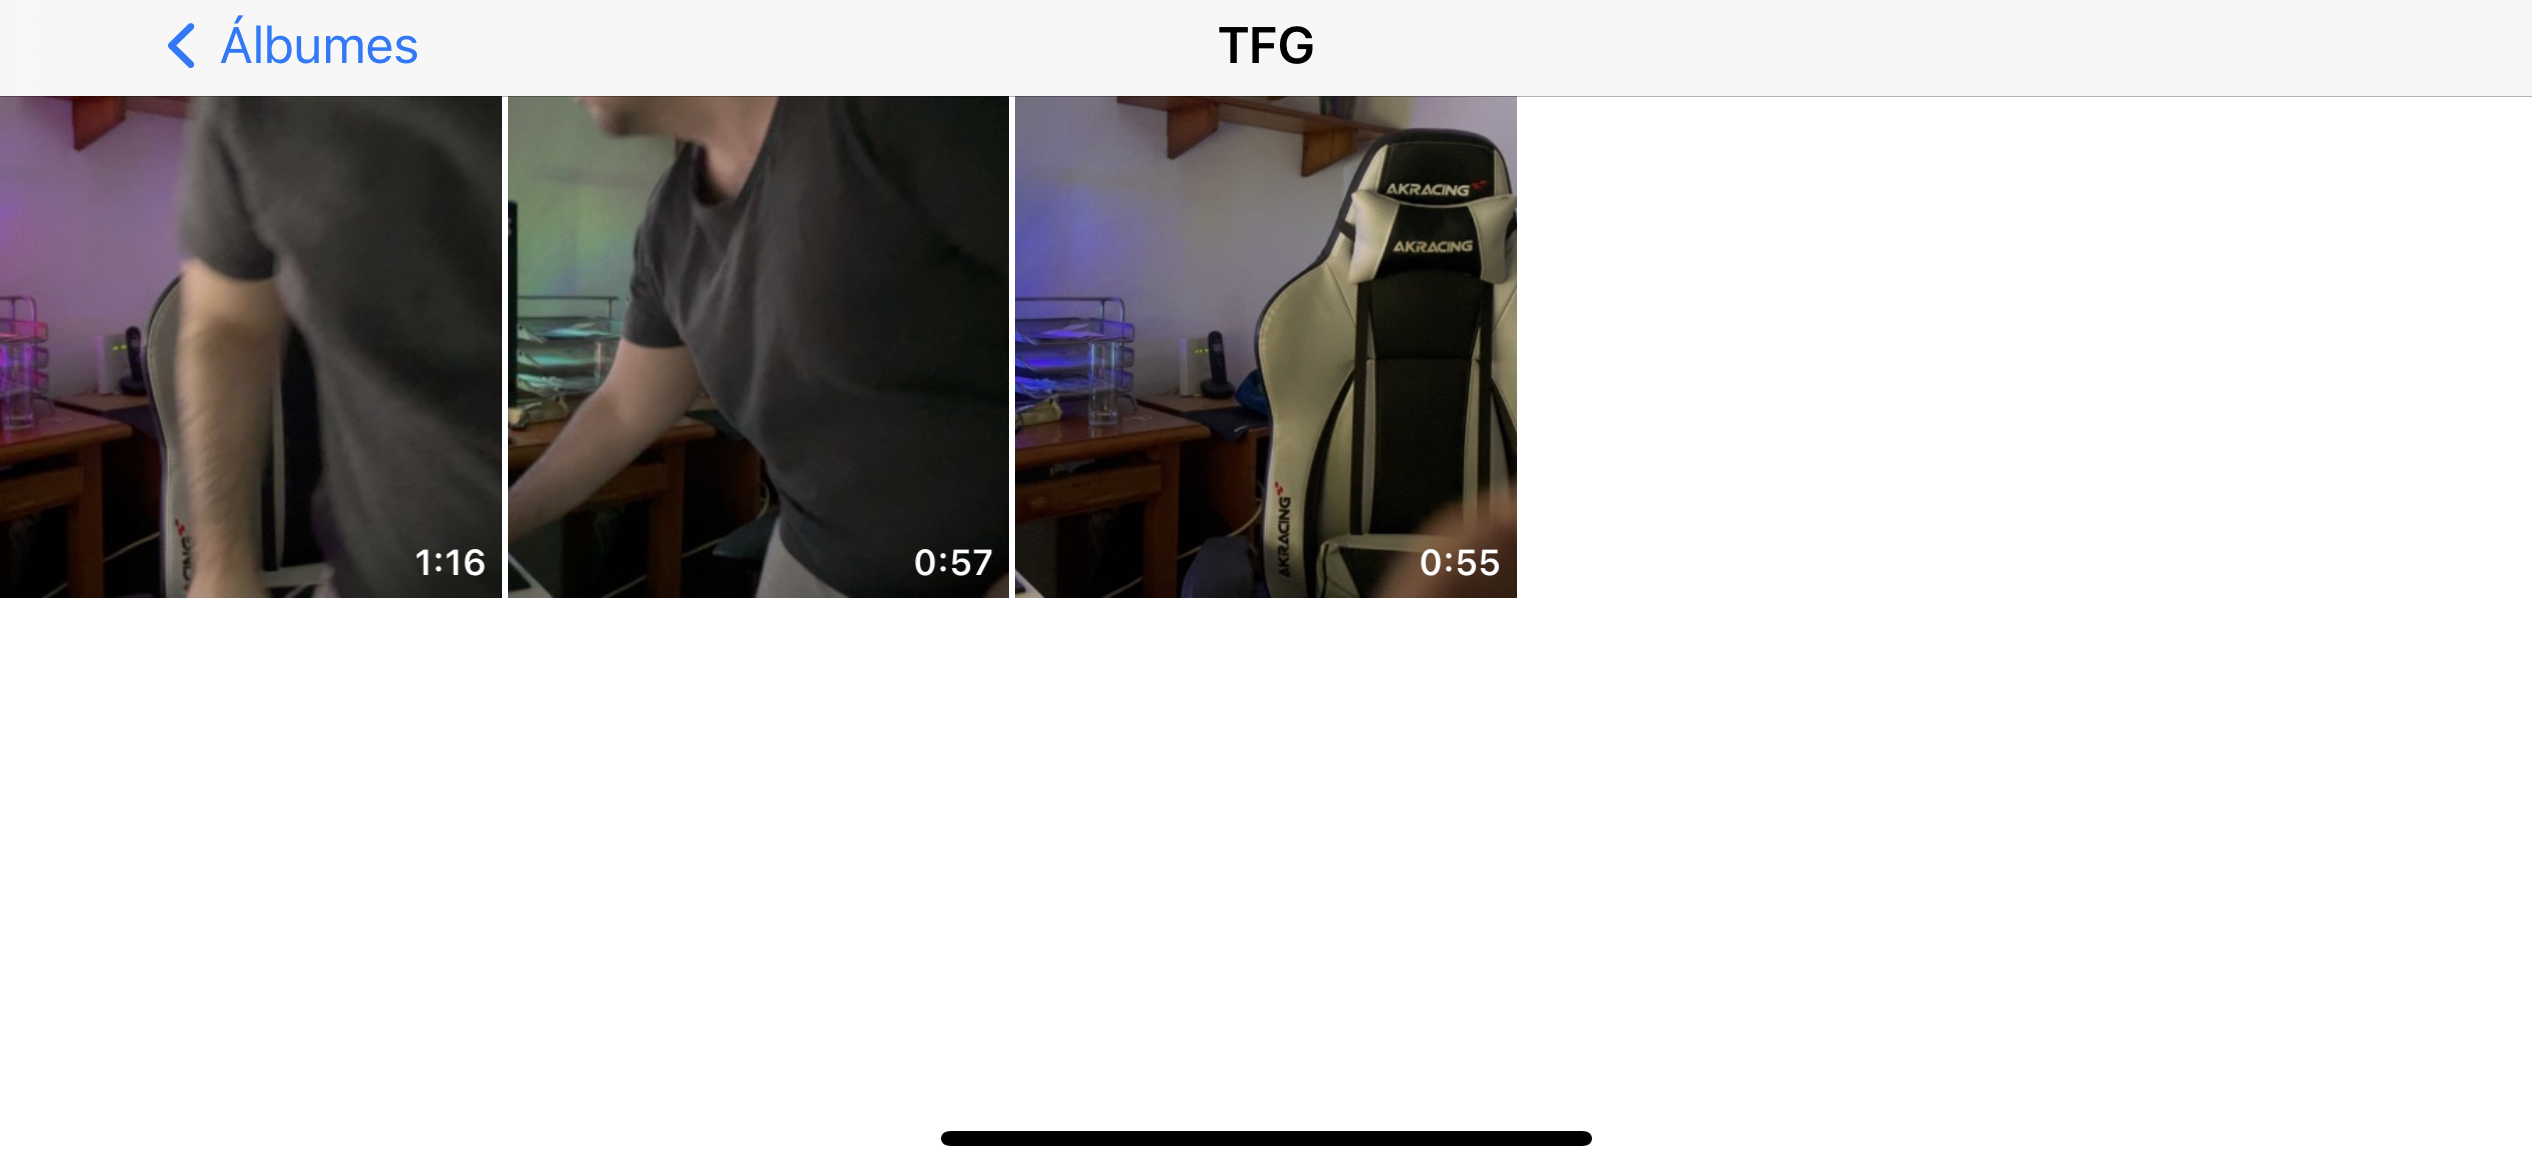
\includegraphics[width=1\textwidth]{images/interpreter/library.PNG}
\caption{Interfaz de selección de vídeos del dispositivo.}
\label{figure21}
\end{figure}

\begin{figure}[h]
\centering 
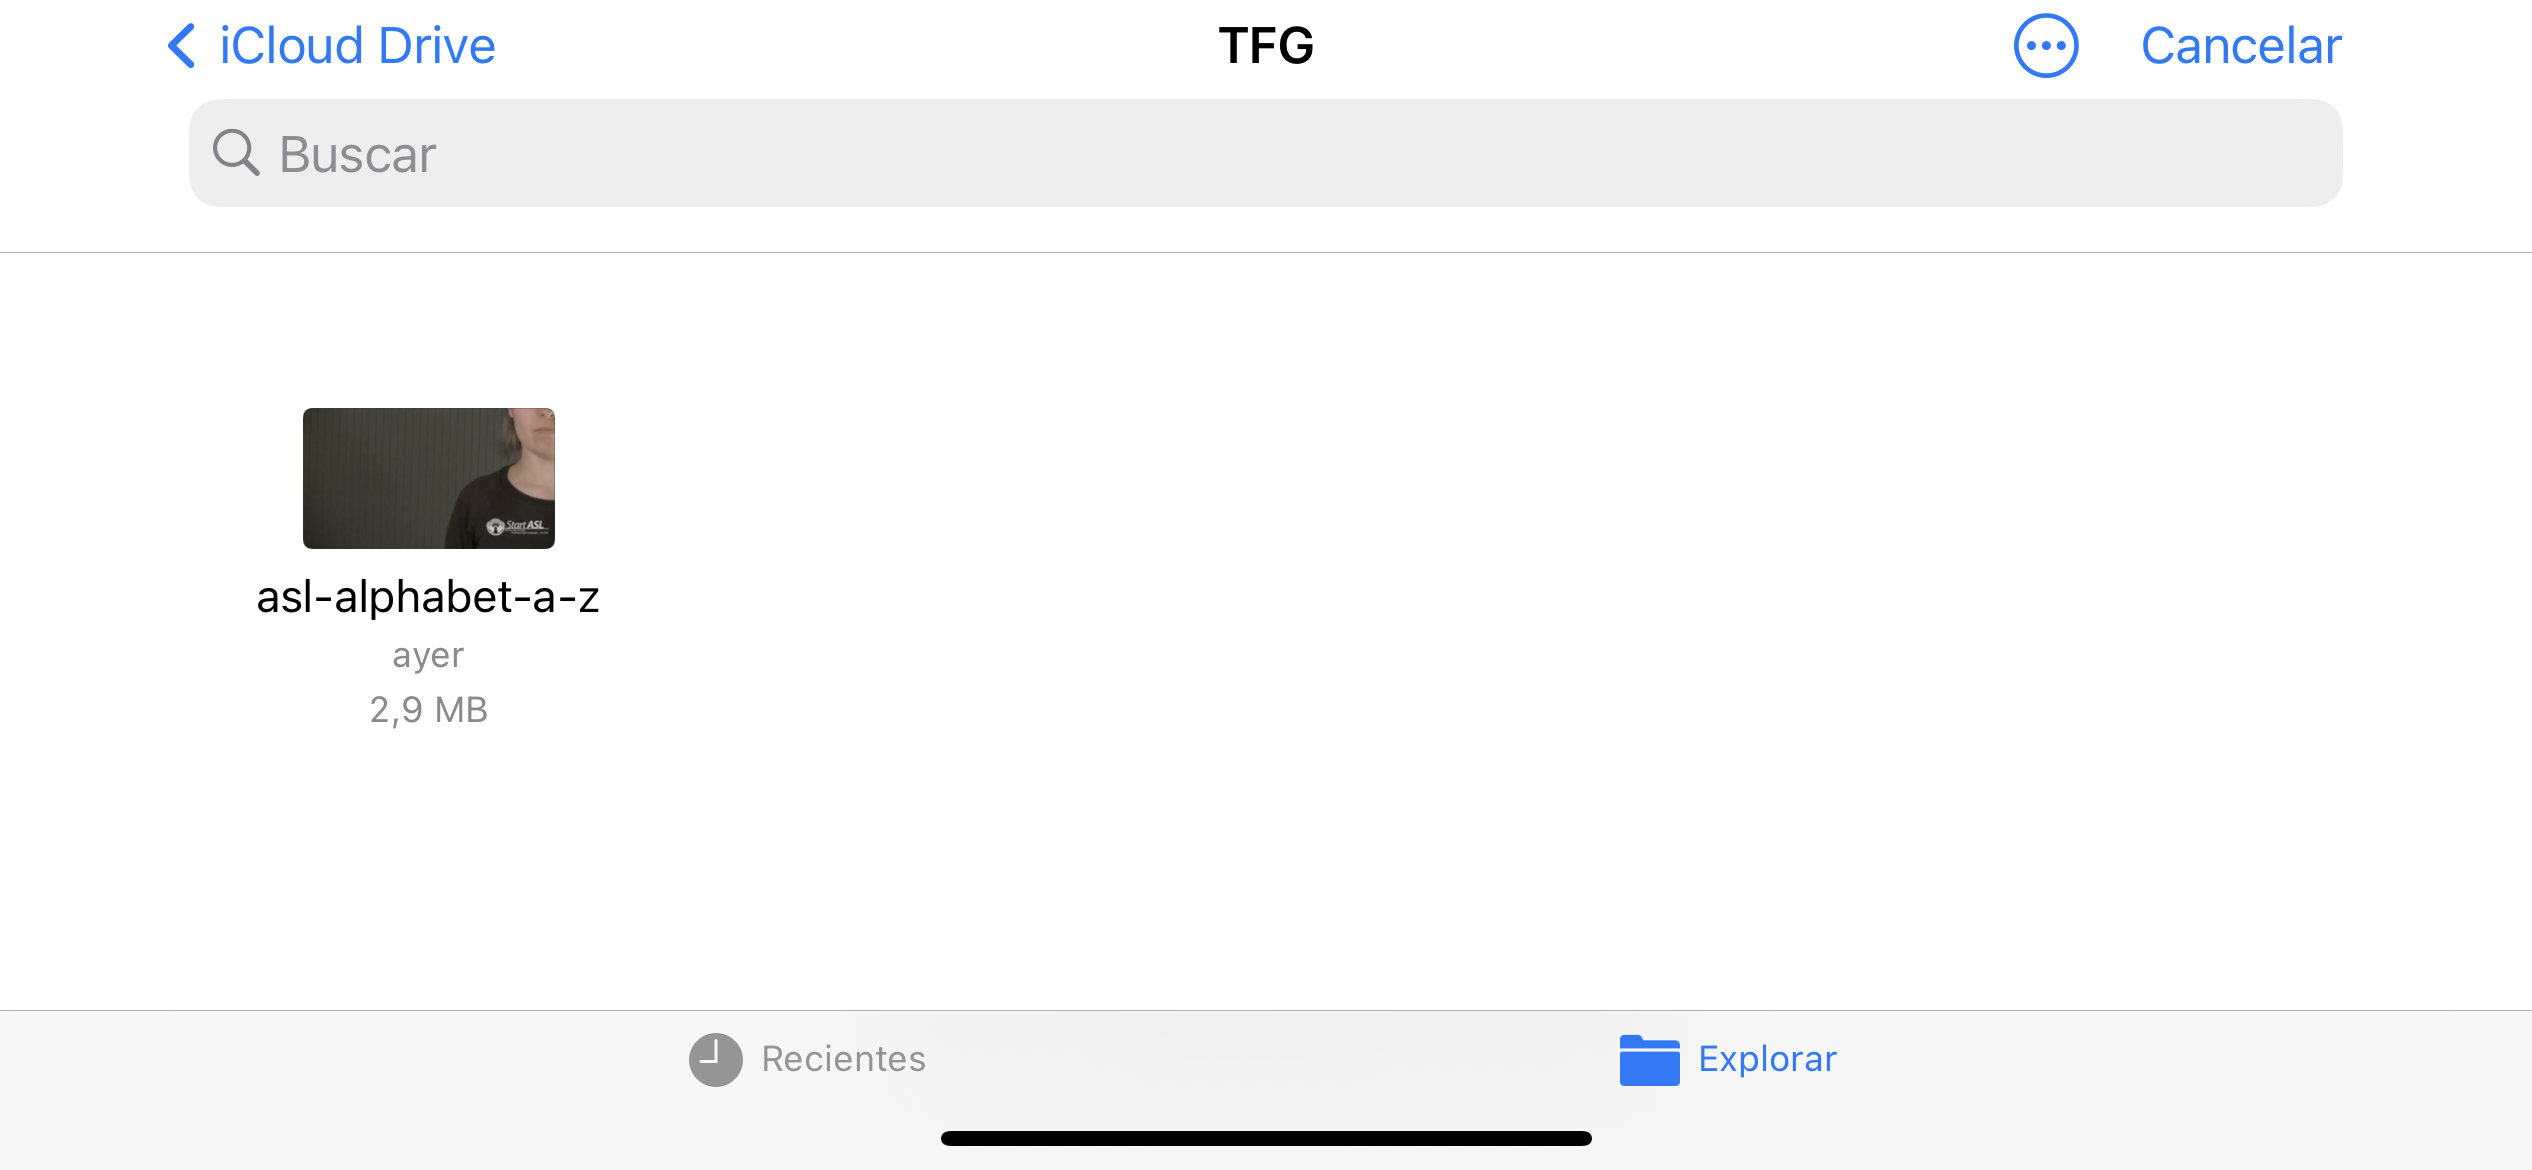
\includegraphics[width=1\textwidth]{images/interpreter/icloud.PNG}
\caption{Interfaz de selección de vídeos desde iCloud.}
\label{figure22}
\end{figure}

\subsection{Camera}

Es la escena encargada de proporcionar un buffer de imágenes para su procesamiento, que puede ser obtenido desde la cámara del dispositivo o desde un fichero de video. Por lo tanto, se distinguen dos modos de funcionamiento:

\begin{itemize}
    \item Cámara del dispositivo: se utiliza la cámara posterior del dispositivo para obtener la mayor calidad de imágen. Se intenta obtener una resolución de 1920x1080. La entrada se mostrará por pantalla utilizando la siguiente clase AVCaptureVideoPreviewLayer. El procesamiento se realizará en segundo plano utilizando una cola para ello.
    
    Se muestran los fragmentos más importante para su configuración:

    
    Queue
    \begin{lstlisting}[style=swift]
    private let cameraQueue = DispatchQueue(label: "CameraDataOutput",
                                           qos: .userInitiated, attributes: [],
                                           autoreleaseFrequency: .workItem)
    \end{lstlisting}
    
    Configuración
    \begin{lstlisting}[style=swift]
        let wideAngle = AVCaptureDevice.DeviceType.builtInWideAngleCamera
        let discoverySession = AVCaptureDevice.DiscoverySession(deviceTypes: [wideAngle],
                                                                mediaType: .video, position: .unspecified)
                                                                
        let session = AVCaptureSession()
        session.beginConfiguration()
        session.sessionPreset = videoDevice.supportsSessionPreset(.hd1920x1080) ? .hd1920x1080 : .high
        
        let dataOutput = AVCaptureVideoDataOutput()
        if session.canAddOutput(dataOutput) {
            session.addOutput(dataOutput)
            dataOutput.alwaysDiscardsLateVideoFrames = true
            dataOutput.videoSettings = [
                String(kCVPixelBufferPixelFormatTypeKey): Int(kCVPixelFormatType_420YpCbCr8BiPlanarFullRange)
            ]
            dataOutput.setSampleBufferDelegate(self, queue: cameraQueue)
        } else {
            showError("can not add output")
        }
    \end{lstlisting}
    
    \item Vídeo: Se obtiene un fichero de vídeo encapsulado en un objeto de tipo AVAsset y se utiliza un objeto de la clase AVPlayer para mostrarlo por pantalla. El video será reproducido inmediatamente tras ser mostrado en pantalla. El procesamiento se realizará en segundo plano utilizando una cola para ello.
    
    Se muestran los fragmentos más importante para su configuración:
    \begin{lstlisting}[style=swift]
    videoFileQueue.async {
            
            // Create sample buffer from pixel buffer
            var sampleBuffer: CMSampleBuffer?
            var formatDescription: CMVideoFormatDescription?
            CMVideoFormatDescriptionCreateForImageBuffer(allocator: nil, imageBuffer: pixelBuffer, formatDescriptionOut: &formatDescription)
            let duration = self.videoFileFrameDuration
            var timingInfo = CMSampleTimingInfo(duration: duration, presentationTimeStamp: itemTime, decodeTimeStamp: itemTime)
            CMSampleBufferCreateForImageBuffer(allocator: nil,
                                               imageBuffer: pixelBuffer,
                                               dataReady: true,
                                               makeDataReadyCallback: nil,
                                               refcon: nil,
                                               formatDescription: formatDescription!,
                                               sampleTiming: &timingInfo,
                                               sampleBufferOut: &sampleBuffer)
            if let sampleBuffer = sampleBuffer {
                self.delegate?.cameraViewController(self, didReceiveBuffer: sampleBuffer, orientation: self.videoFileBufferOrientation)
            }
        }
    }
    \end{lstlisting}
\end{itemize}
    Esta clase actúa como delegado del intérprete y se encarga de transmitir un buffer de imágenes. Para ello, se utiliza el siguiente protocolo:
    
    \begin{lstlisting}[style=swift]
    protocol CameraViewControllerDelegate: class {
        func cameraViewController(_ controller: CameraViewController, didReceiveBuffer buffer: CMSampleBuffer, orientation: CGImagePropertyOrientation)
    }
    \end{lstlisting}

\subsection{Interpreter ASL}

Es la escena principal de la aplicación y del proyecto. Se encarga de realizar predicciones utilizando como entrada un buffer de imágenes y mostrando por pantalla los resultados. Se compone de los siguientes modos de funcionamiento que pueden configurarse en la escena de configuración:

\begin{itemize}
    \item Free \label{free}: Muestra por pantalla los resultados obtenidos de las predicciones sin ningún procesamiento posterior. Es una vista en tiempo real de las predicciones devueltas por el modelo de Deep Learning.
    \item Letter occurrences\label{occurrences}: Tras obtener una predicción, se realiza un proceso de refinamiento para obtener resultados más fiables. Para confirmar una predicción como correcta, se requieren un mínimo número de predicciones consecutivas con el mismo resultado. Puede configurarse obtener varias predicciones consecutivas iguales o un mínimo de ocurrencias sobre un total. Por ejemplo, 5 de 6 predicciones de la misma letra para confirmarse como correcta. Estos parámetros "Minimum letters to compare results" y "Minimum occurrences of letters detected" pueden ser configurados en la escena de configuración.
    \item Detect words\label{words}: Se encarga de ir formando palabras con las letras detectadas. También utiliza el proceso de refinamiento comentado anteriormente para mejorar los resultados. A medida que se detectan letras se muestran por pantalla formando una palabra hasta que se decide que la palabra ha terminado. Para interpretar cuando una palabra empieza y acaba, se necesita un procesamiento adicional. Mediante un gesto con la mano, podremos indicar cuando una palabra empieza y acaba.
\end{itemize}

La interfaz cuenta con los siguientes elementos que pueden visualizarse en la figura \ref{figure23}:

\begin{itemize}
    \item En la esquina inferior izquierda se muestran las 3 predicciones con la mayor probabilidad de ser correcta. Estos son los resultados devueltos por el modelo de Deep Learning en tiempo real sin ningún procesamiento. Estos resultados son sólo visibles en modo depuración,  esto puede establecerse en la escena de configuración.
    \item En la esquina inferior derecha se muestra la letra con la probabilidad más alta detectada en el caso de que se haya confirmado como correcta. Según el modo de funcionamiento se pueden necesitar varias predicciones consecutivas de la misma letra para confirmarse. En caso de que no se confirme ninguna letra esta vista no será visible o contendrá los últimos resultados válidos.
    \item Bounding Box: Rectángulo para visualizar la mano que se ha utilizado para la predicción. En la escena de configuración podemos elegir si se utiliza la mano izquierda o derecha. 
\end{itemize}

El código completo es bastante extenso así que se van a mostrar las configuraciones más importantes.

El primer paso es detectar la mano es una imagen, para ello seguiremos el mismo procedimiento que se utilizó en la aplicación de entrenamiento para la extracción de características. Utilizamos Vision Framework, y mediante la petición VNDetectHumanHandPoseRequest se obtiene la detección de hasta dos manos en una imagen.

\begin{lstlisting}[style=swift]
override func viewDidAppear(_ animated: Bool) {
        super.viewDidAppear(animated)
        handPoseRequest = VNDetectHumanHandPoseRequest()
        handPoseRequest.maximumHandCount = 2
}
   
 func checkObservations(_ controller: CameraViewController, buffer: CMSampleBuffer, orientation: CGImagePropertyOrientation) throws {
    let visionHandler = VNImageRequestHandler(cmSampleBuffer: buffer, orientation: orientation, options: [:])
    try visionHandler.perform([handPoseRequest]) 
\end{lstlisting}

Se utiliza el mismo modelo y proceso para la obtención y normalización de coordenadas que la aplicación de entrenamiento. El modelo Hand es el mismo en ambas aplicaciones.  
\begin{lstlisting}[style=swift]
func processObservations(_ observation: VNHumanHandPoseObservation) -> Hand? {
    guard observation.confidence >= minConfidenceObservation else {
        print("observation low confidence")
        return nil
    }
    
    do {
           
        let wrist = try observation.recognizedPoint(.wrist)
        let indexFingerPoints = try observation.recognizedPoints(.indexFinger)
        let ringFingerPoints = try observation.recognizedPoints(.ringFinger)
        let thumbFingerPoints = try observation.recognizedPoints(.thumb)
        let littleFingerPoints = try observation.recognizedPoints(.littleFinger)
        let middleFingerPoints = try observation.recognizedPoints(.middleFinger)
        
        let hand = HandFingerPoints(indexFingerPoints: indexFingerPoints,
                                    ringFingerPoints: ringFingerPoints,
                                    littleFingerPoints: littleFingerPoints,
                                    middleFingerPoints: middleFingerPoints,
                                    thumbFingerPoints: thumbFingerPoints,
                                    wristPoint: wrist)
        
        hand.normalizeHand()
        numberOfProcess += 1
        return hand
    } catch {
        print(error)
        return nil
    }
}
\end{lstlisting}

Sobre el modelo obtenido, realizamos la extracción de características que consiste en obtener una array de 42 valores de tipo Double que representan la posición relativa de diferentes posiciones de la mano. El método extractIfValidFeatures recibe un parámetro que indica si debemos invertir el valor de las coordenadas del eje X. 

EL modelo ha sido entrenado en su totalidad con fotos de la mano derecha de diferentes personas. Para mejorar los resultados es importante que tanto los datos de entrenamiento como los datos de entrada para realizar una predicción sean sobre la misma mano. Sin embargo, podemos realizar también predicciones con la mano izquierda con tan sólo invertir los valores del eje X. Todas las coordenadas están normalizadas de 0.0 a 1.0, así que para invertir el valor de una posición simplemente restamos a 1.0 el valor correspondiente. La mano utilizada para realizar la predicción puede ser configurada en la escena de configuración.

Como respuesta del método 'prediction(multiArrayBuffer: multiArrayBuffer)', obtenemos una distribución de probabilidad. Se filtran las 3 predicciones con mayor probabilidad y se muestran por pantalla. También se obtiene el mejor resultado para su procesamiento. El Interactor será el encargado de recibir la letra detectada y volverá a comunicarse con el Intérprete para transmitir el resultado, en caso de que la predicción se confirme como correcta.

\begin{lstlisting}[style=swift]
guard let hand = VisionProcessImage.sharedInstance.processObservations(observation),
    let features = hand.extractIfValidFeatures(flipX: ASLConfiguration.shared.handCase == ASLConfiguration.HandCase.left) else {
    print("failed to extract hand features")
    return
}
if let multiArrayBuffer = try? MLMultiArray(features) {
    let labelProbability = ASLConfiguration.shared.prediction(multiArrayBuffer: multiArrayBuffer)
    let top3 = labelProbability.sorted {
        return $0.value > $1.value
    }.prefix(3)
    
    let descriptionTop3 = top3.map { observation in
        String(format: "%@ %.1f%%", observation.key, observation.value * 100)}
    DispatchQueue.main.async {
        if ASLConfiguration.shared.isDebugMode {
            self.aslView.labelResults.text = descriptionTop3.joined(separator: "\n")
        }
    }
    
    if let betterPrediction = top3.first, betterPrediction.value > Double(ASLConfiguration.shared.letterDetectionMinConfidence) {
        interactor?.topPredictionLetter(betterPrediction.key)
    }
}
\end{lstlisting}



\begin{figure}[h]
\centering 
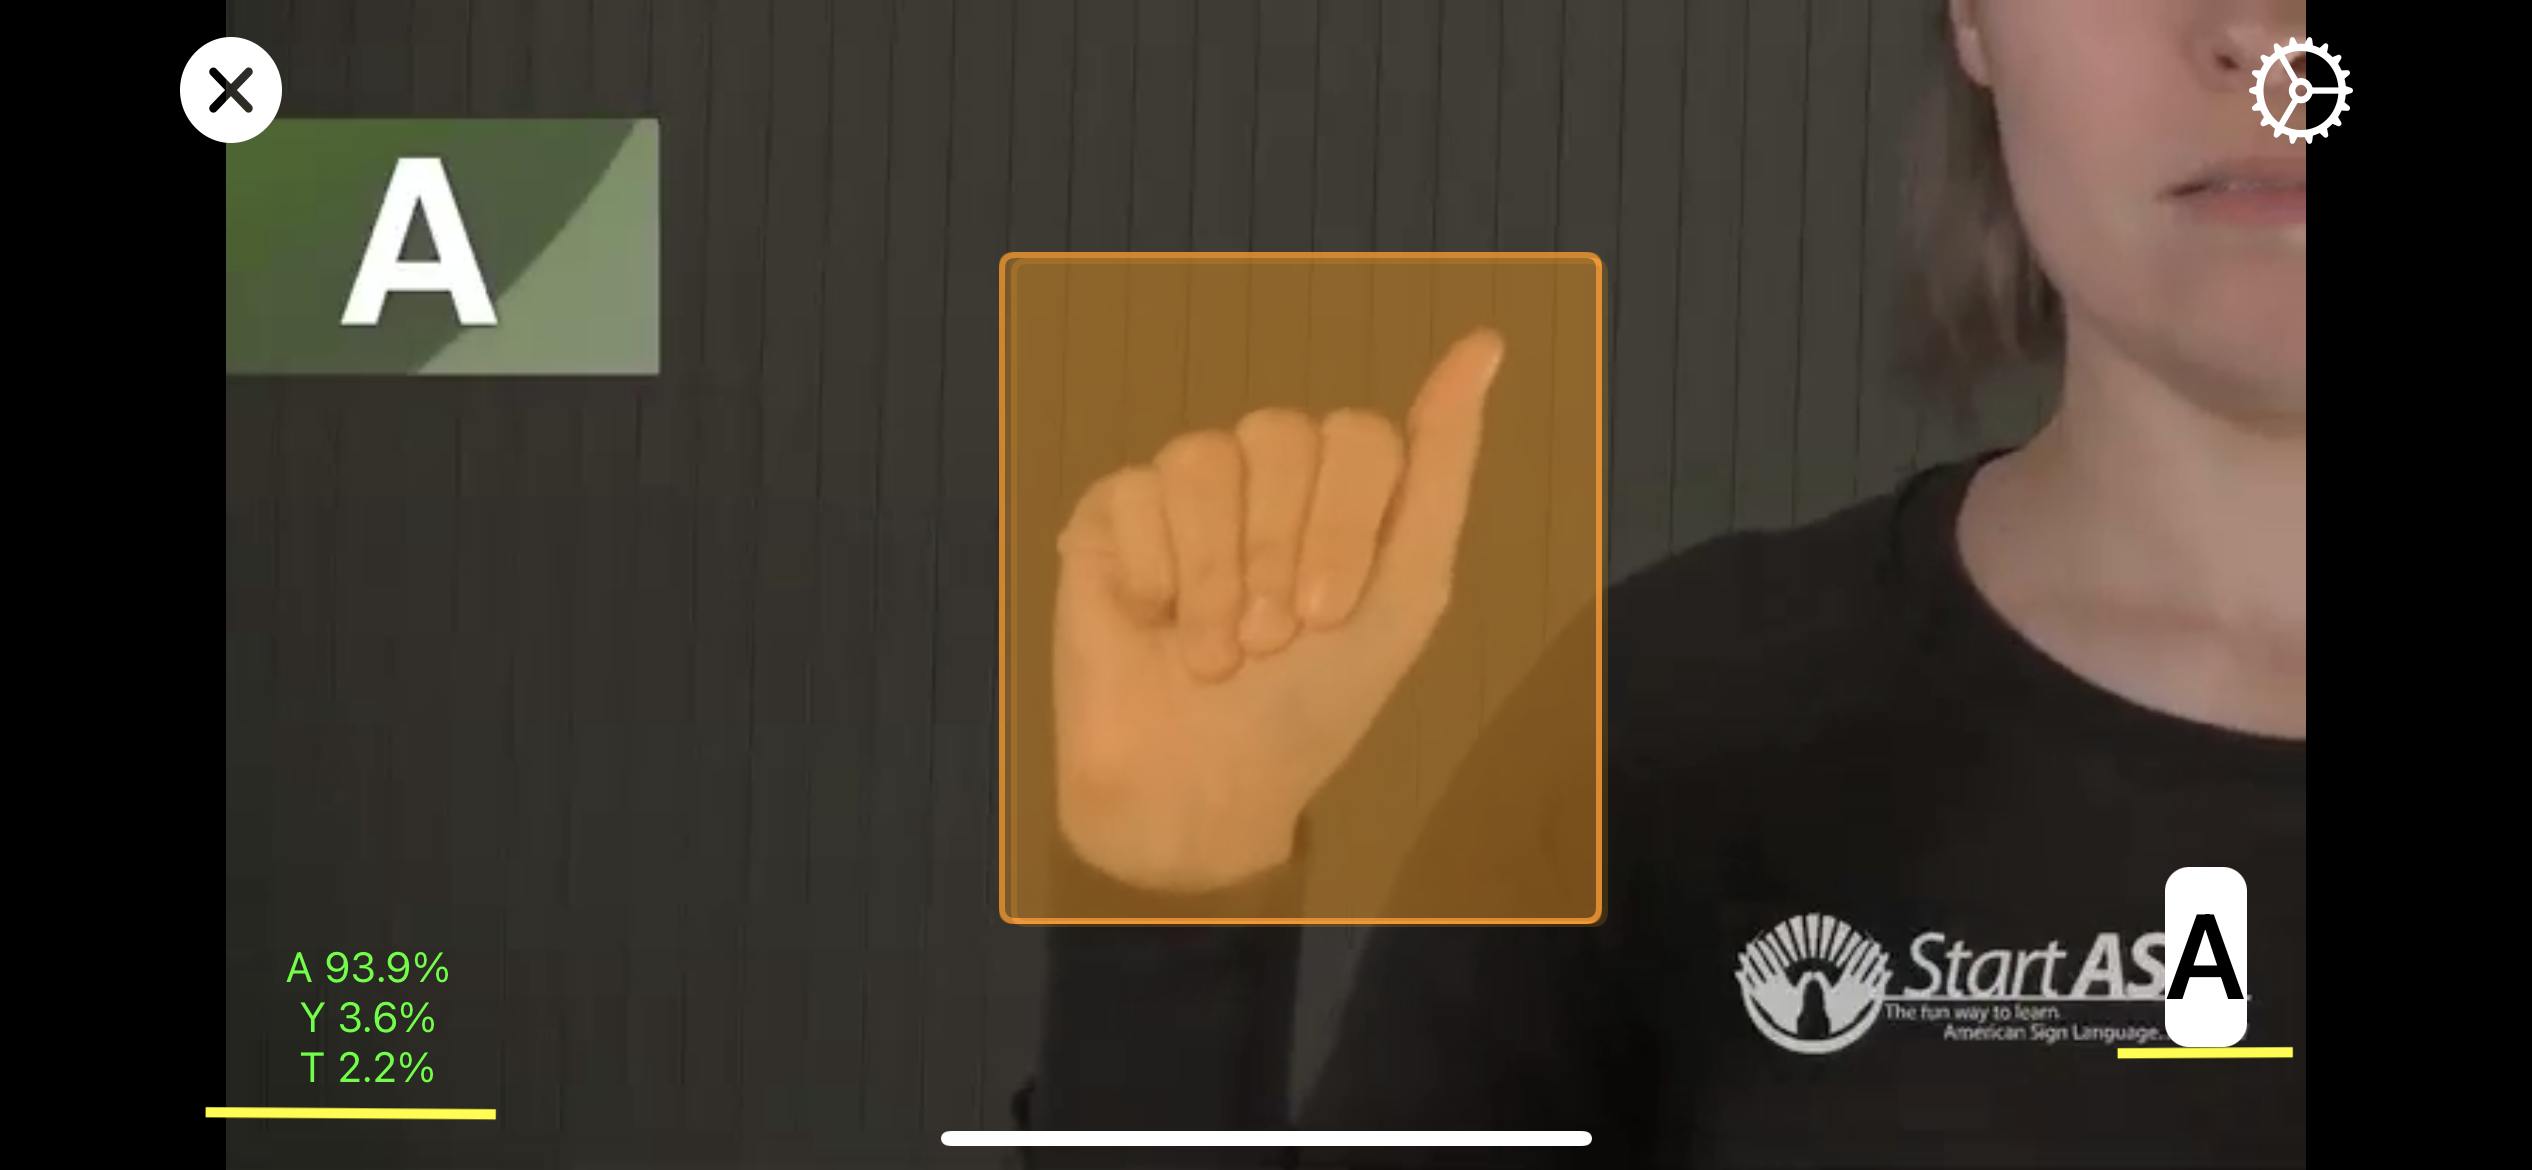
\includegraphics[width=1\textwidth]{images/interpreter/asl1.PNG}
\caption{Interfaz intérprete ASL.}
\label{figure23}
\end{figure}

La clase ASLInterpreterWorker es la encargada de confirmar una predicción como correcta o no. Esto dependerá del modo de funcionamiento de la aplicación así como de los diferentes parámetros establecidos. En el modo de funcionamiento Free \ref{free}, siempre devolverá una predicción como correcta. En el modo de funcionamiento Letter Occurrences \ref{occurrences}, se trata de confirmar si de las últimas X predicciones, al menos Y son de la misma letra. En este caso, esta letra se confirma como correcta.
\begin{lstlisting}[style=swift]
func detectMinOcurrencesLetter(_ letter: String) {
    queue.async { [unowned self] in
        self.predictions.append(letter)
        
        if predictions.count >= ASLConfiguration.shared.minLettersToCompare {
            let slide = predictions.suffix(ASLConfiguration.shared.minLettersToCompare)
            let lastPredictions = Array(slide)
            
            let occurences: [Occurrence] = getNumberOfOccurrences(lastLetters: lastPredictions)
            guard let topResult = getTopResult(ocurrences: occurences) else {
                return
            }
            
            if topResult.times >= ASLConfiguration.shared.minOcurrences && topResult.letter != lastLetter {
                lastLetter = topResult.letter
                predictions.removeAll()
                delegate?.aslInterpreter(self, didDetectWord: topResult.letter)
            }
        }
    }
}
\end{lstlisting}    

\begin{figure}[h]
\centering 
\includegraphics[width=1\textwidth]{images/interpreter/asl2.PNG}
\caption{Interfaz intérprete ASL.}
\label{figure24}
\end{figure}

\begin{figure}[h]
\centering 
\includegraphics[width=1\textwidth]{images/interpreter/asl3.PNG}
\caption{Interfaz intérprete ASL.}
\label{figure25}
\end{figure}

Para el modo de funcionamiento Detect Words \ref{words}, se necesita configuración adicional. Necesitamos detectar cuándo  empieza y termina una palabra. Para ello, vamos a utilizar un detector de gestos. El procedimiento es el siguiente:

Se utilizará una mano para las representación de las letras, y la otra mano para realizar un gesto. Por tanto ambas manos necesitan estar visibles para este modo de funcionamiento. En caso de seleccionar en la escena de configuración la mano derecha, se utilizará la mano izquierda para interpretar el gesto.

El gesto utilizado para indicar cuando empieza y termina una palabra es denominado Pinch. Consiste en tener los dedos índices y pulgar juntos. Se detecta la posición de los dedos índices y pulgar, y dependiendo si la distancia entre ellos es inferior a un valor mínimo, se considera que se encuentra en un estado Pinch \ref{figure26}, en el caso contrario, el estado es apart \ref{figure27}.

\begin{lstlisting}[style=swift]
guard let middlePoints = try? rightHand.recognizedPoints(.thumb),
      let indexFingerPoints = try? rightHand.recognizedPoints(.indexFinger),
      let middleTipPoint = middlePoints[.thumbTip],
      let indexTipPoint = indexFingerPoints[.indexTip] else {
    return
}
    
let minConfidenceFinger: VNConfidence = 0.3
guard middleTipPoint.confidence > minConfidenceFinger && indexTipPoint.confidence > minConfidenceFinger else {
    return
}

let thumbTip = middleTipPoint.location.applying(.verticalFlip)
let indexTip = indexTipPoint.location.applying(.verticalFlip)

let thumbTipLayer = controller.viewPointForVisionPoint(thumbTip)
let indexTipLayer = controller.viewPointForVisionPoint(indexTip)
gestureProcessor.newPoints(thumbTip: thumbTipLayer, indexTip: indexTipLayer)
\end{lstlisting}

La clase HandGestureProcessor es la encargada de ir recibiendo estos dos puntos y determinar en el estado se encuentra:
\begin{enumerate}
    \item possiblePinch: Se han detectado evidencias de que se ha realizado un gesto pinch, pero no se han alcanzado en mínimo número de evidencias para confirmarlo.
    \item pinched: se ha confirmado que se encuentra en el estado pinched. 
    \item possibleApart: partiendo del estado pinched, se ha detectado alguna evidencia de que los dedos no están lo suficientemente juntos, pero aún no esta confirmado.
    \item apart: Se ha realizado la transición del estado pinched al estado apart, se detecta como el fin de una palabra.
    \item unknown: No determinado. Si pasan más de dos segundos sin recibir ninguna información o aún no se ha recibido ninguna información, se encuentra en este estado. 
\end{enumerate}

Definición de estados:

\begin{lstlisting}[style=swift]
enum State {
    case possiblePinch
    case pinched
    case possibleApart
    case apart
    case unknown
}
\end{lstlisting}

\begin{figure}[h]
\centering 

\includegraphics[width=0.6\textwidth]{images/interpreter/pinch.png}
\caption{Estado pinched.}
\label{figure26}
\end{figure}

\begin{figure}[h]
\centering 
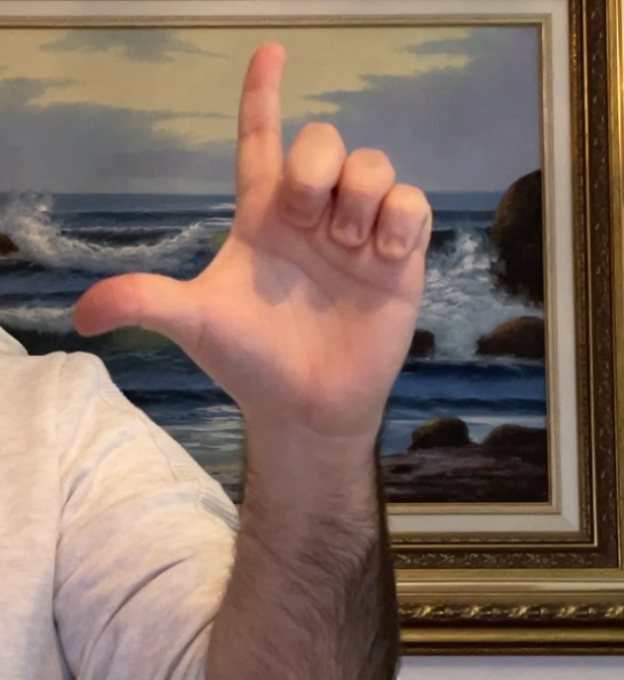
\includegraphics[width=0.6\textwidth]{images/interpreter/apart.png}
\caption{Estado apart.}
\label{figure27}
\end{figure}


Según una distancia mínima establecida pinchMaxDistance, se modifica el estado actual. 
\begin{lstlisting}[style=swift]
func newPoints(thumbTip: CGPoint, indexTip: CGPoint) {
    lastEventDate = Date()
    let distance = indexTip.distance(from: thumbTip)
    if distance < pinchMaxDistance {
        pinchEvidenceCounter += 1
        apartEvidenceCounter = 0
        state = (pinchEvidenceCounter >= evidenceCounterStateTrigger) ? .pinched : .possiblePinch
    } else {
        apartEvidenceCounter += 1
        pinchEvidenceCounter = 0
        state = (apartEvidenceCounter >= evidenceCounterStateTrigger) ? .apart : .possibleApart
    }
}
\end{lstlisting}

La aplicación sólo realiza predicciones sobre el modelo de Deep Learning si se encuentra entre los estados possiblePinch, pinched o possibleApart. En caso contrario, únicamente se intenta identificar si se ha realizado un gesto Pinch.

Cuando se confirma el estado apart, se confirma el fin de una palabra. Al establecer el fin de una palabra, en la siguiente predicción, se eliminaran los resultados anteriores de la pantalla y se empieza una palabra sin ninguna  letra anterior.


\begin{lstlisting}[style=swift]
if ASLConfiguration.shared.isTextCheckerEnabled {
    print("textChecking")
    var newWord = word.joined()
    let language = "en"
    let rangeMisspelled = textChecker.rangeOfMisspelledWord(in: newWord, range: NSRange(0..<newWord.utf16.count), startingAt: 0, wrap: false, language: language)
    if rangeMisspelled.location != NSNotFound {
        if let guess = textChecker.guesses(forWordRange: rangeMisspelled, in: newWord, language: language)?.first {
            newWord = guess
            print("newWord: guess: \(guess)")
        }
    }
    delegate?.aslInterpreter(self, didDetectWord: newWord)
}
\end{lstlisting}

\subsection{Configuración}

Por último, tenemos una escena de configuración, a la cual se puede acceder desde cualquier escena y que permite cambiar diferentes parámetros que son utilizados por la aplicación. Se puede pausar la ejecución de cualquier video o cámara, cambiar los parámetros y continuar por el mismo punto con los nuevos parámetros actualizados. La interfaz se puede ver en la figura \ref{figure28} y \ref{figure29}.

Los parámetros son los siguientes:
\begin{enumerate}
    \item Minimal hand confidence: Es usado para la detección de una mano en una imagen. Se utiliza para filtrar los resultados obtenidos por Vision Framework \cite{Vision}. Las predicciones con un nivel de confianza menor al establecido son descartadas.
    \item Minimal letter confidence: Es usado para la detección de letras sobre el modelo de Deep Learning. Cualquier predicción con un nivel de confianza inferior es descartado.
    \item Mode: Define el modo de funcionamiento de la aplicación. Los modos son definidos en el punto \ref{free}.
    \item Minimum letters to compare results: Se utiliza para el modo de funcionamiento Letter occurrences y Detect Words. Determina el mínimo número de predicciones necesarias antes de poder confirmar una predicción como correcta.
    \item Minimum occurrences of letters detected: Se utiliza para el modo de funcionamiento Letter occurrences y Detect Words. Determina el mínimo número de ocurrencias de una misma letra sobre las últimas predicciones para confirmar la letra como correcta. 
    \item Filter hand by mid X coordinate: En caso de estar habilitado, si estamos realizando predicciones sobre la mano derecha, la mano necesita estar localizada en la primera mitad de la pantalla sobre el eje horizontal, en caso contrario es rechazada. Si es con la mano izquierda es en sentido inverso. Esto sirve para rechazar predicciones erróneas en las transiciones entre letras. Para un buen funcionamiento bajo este modo, es necesario que la persona que realiza los gestos esté centrada en la imagen.
    \item Hand: Permite seleccionar la mano sobre la que se realizarán predicciones. En caso de solo ser visible una mano, se utiliza sin importar cual esté seleccionada en este parámetro.
    \item Modelo: Parámetro utilizado para el desarrollo del proyecto. Permite seleccionar entre diferentes modelos de Deep Learning que se han ido desarrollando en diferentes iteraciones del proyecto. El modelo seleccionado por defecto es el que tiene los mejores resultados con un porcentaje del 95\% de precisión en el test de validación.
    \item Debug: En caso de estar habilitado, imprime diferentes mensajes por pantalla para ayudar en el desarrollo. Así como habilita la vista de resultados en tiempo real, esta vista se puede ver en la figura \ref{figure25}.
    \item Resets to defaults: Restaurar todos los parámetros a su configuración inicial.
\end{enumerate}

La configuración inicial es la que ha dado mejores resultados, especialmente para la confirmación de predicciones, obtener 6 predicciones consecutivas de la misma letra es un buen indicador de que es una buena predicción. Esto puede provocar que alguna vez se rechace alguna predicción que es correcta, pero devuelve los mejores resultados para tener un buen balance y evitar predicciones erróneas que pueden producirse entre transiciones entre letras o por pequeñas variaciones en la mano.


\begin{figure}[h]
\centering 
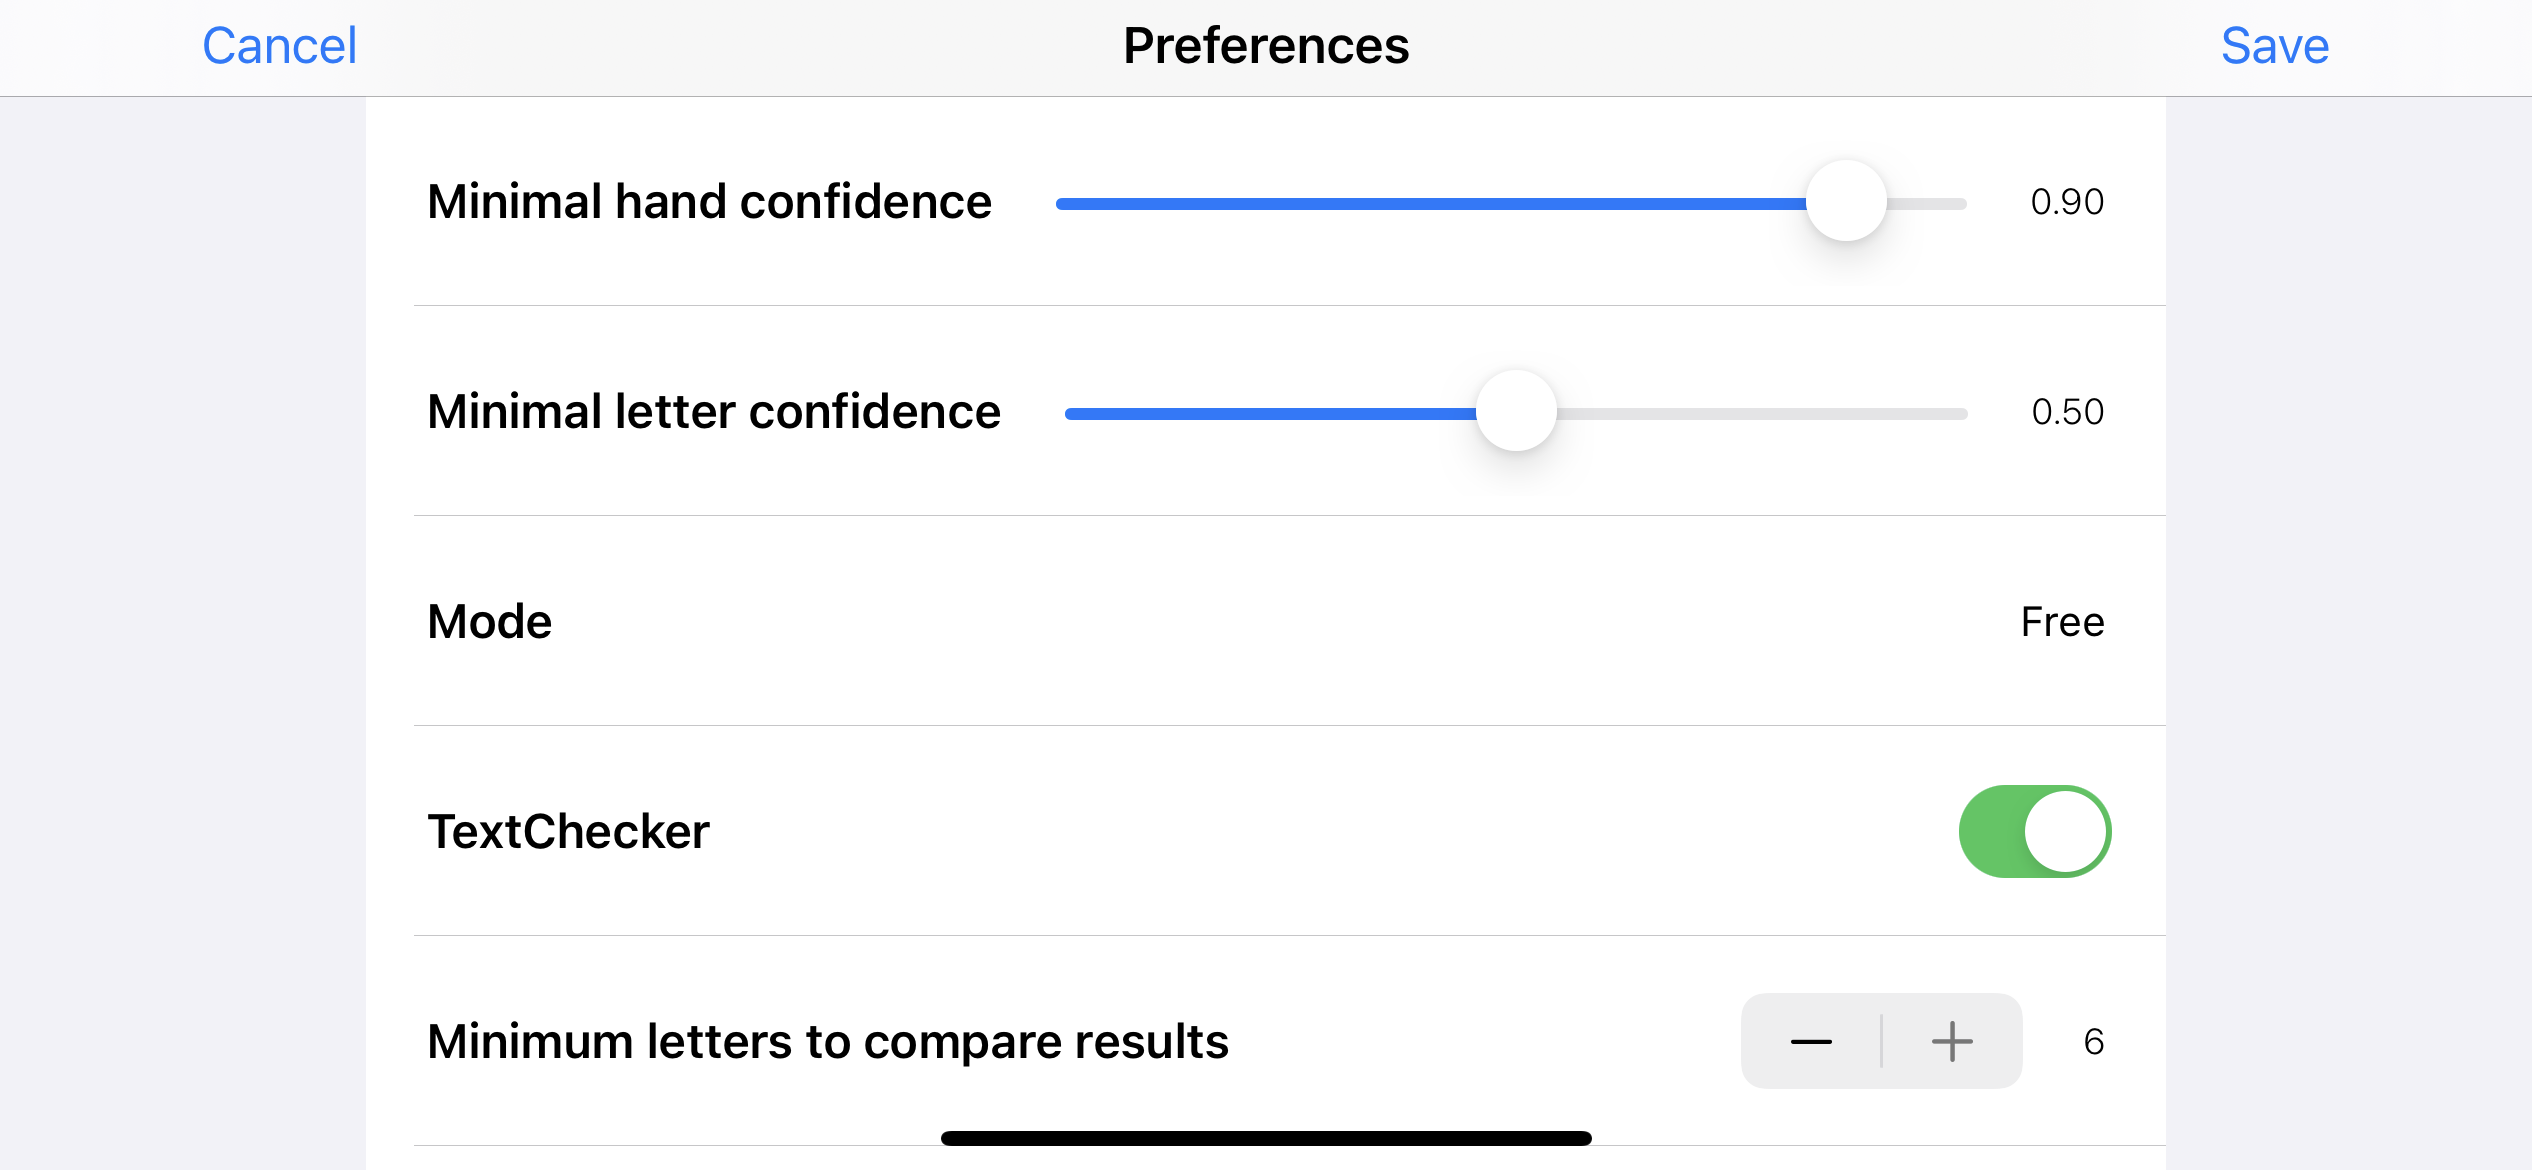
\includegraphics[width=1\textwidth]{images/interpreter/config-scene1.PNG}
\caption{Parámetros de configuración.}
\label{figure28}
\end{figure}

\begin{figure}[h]
\centering 
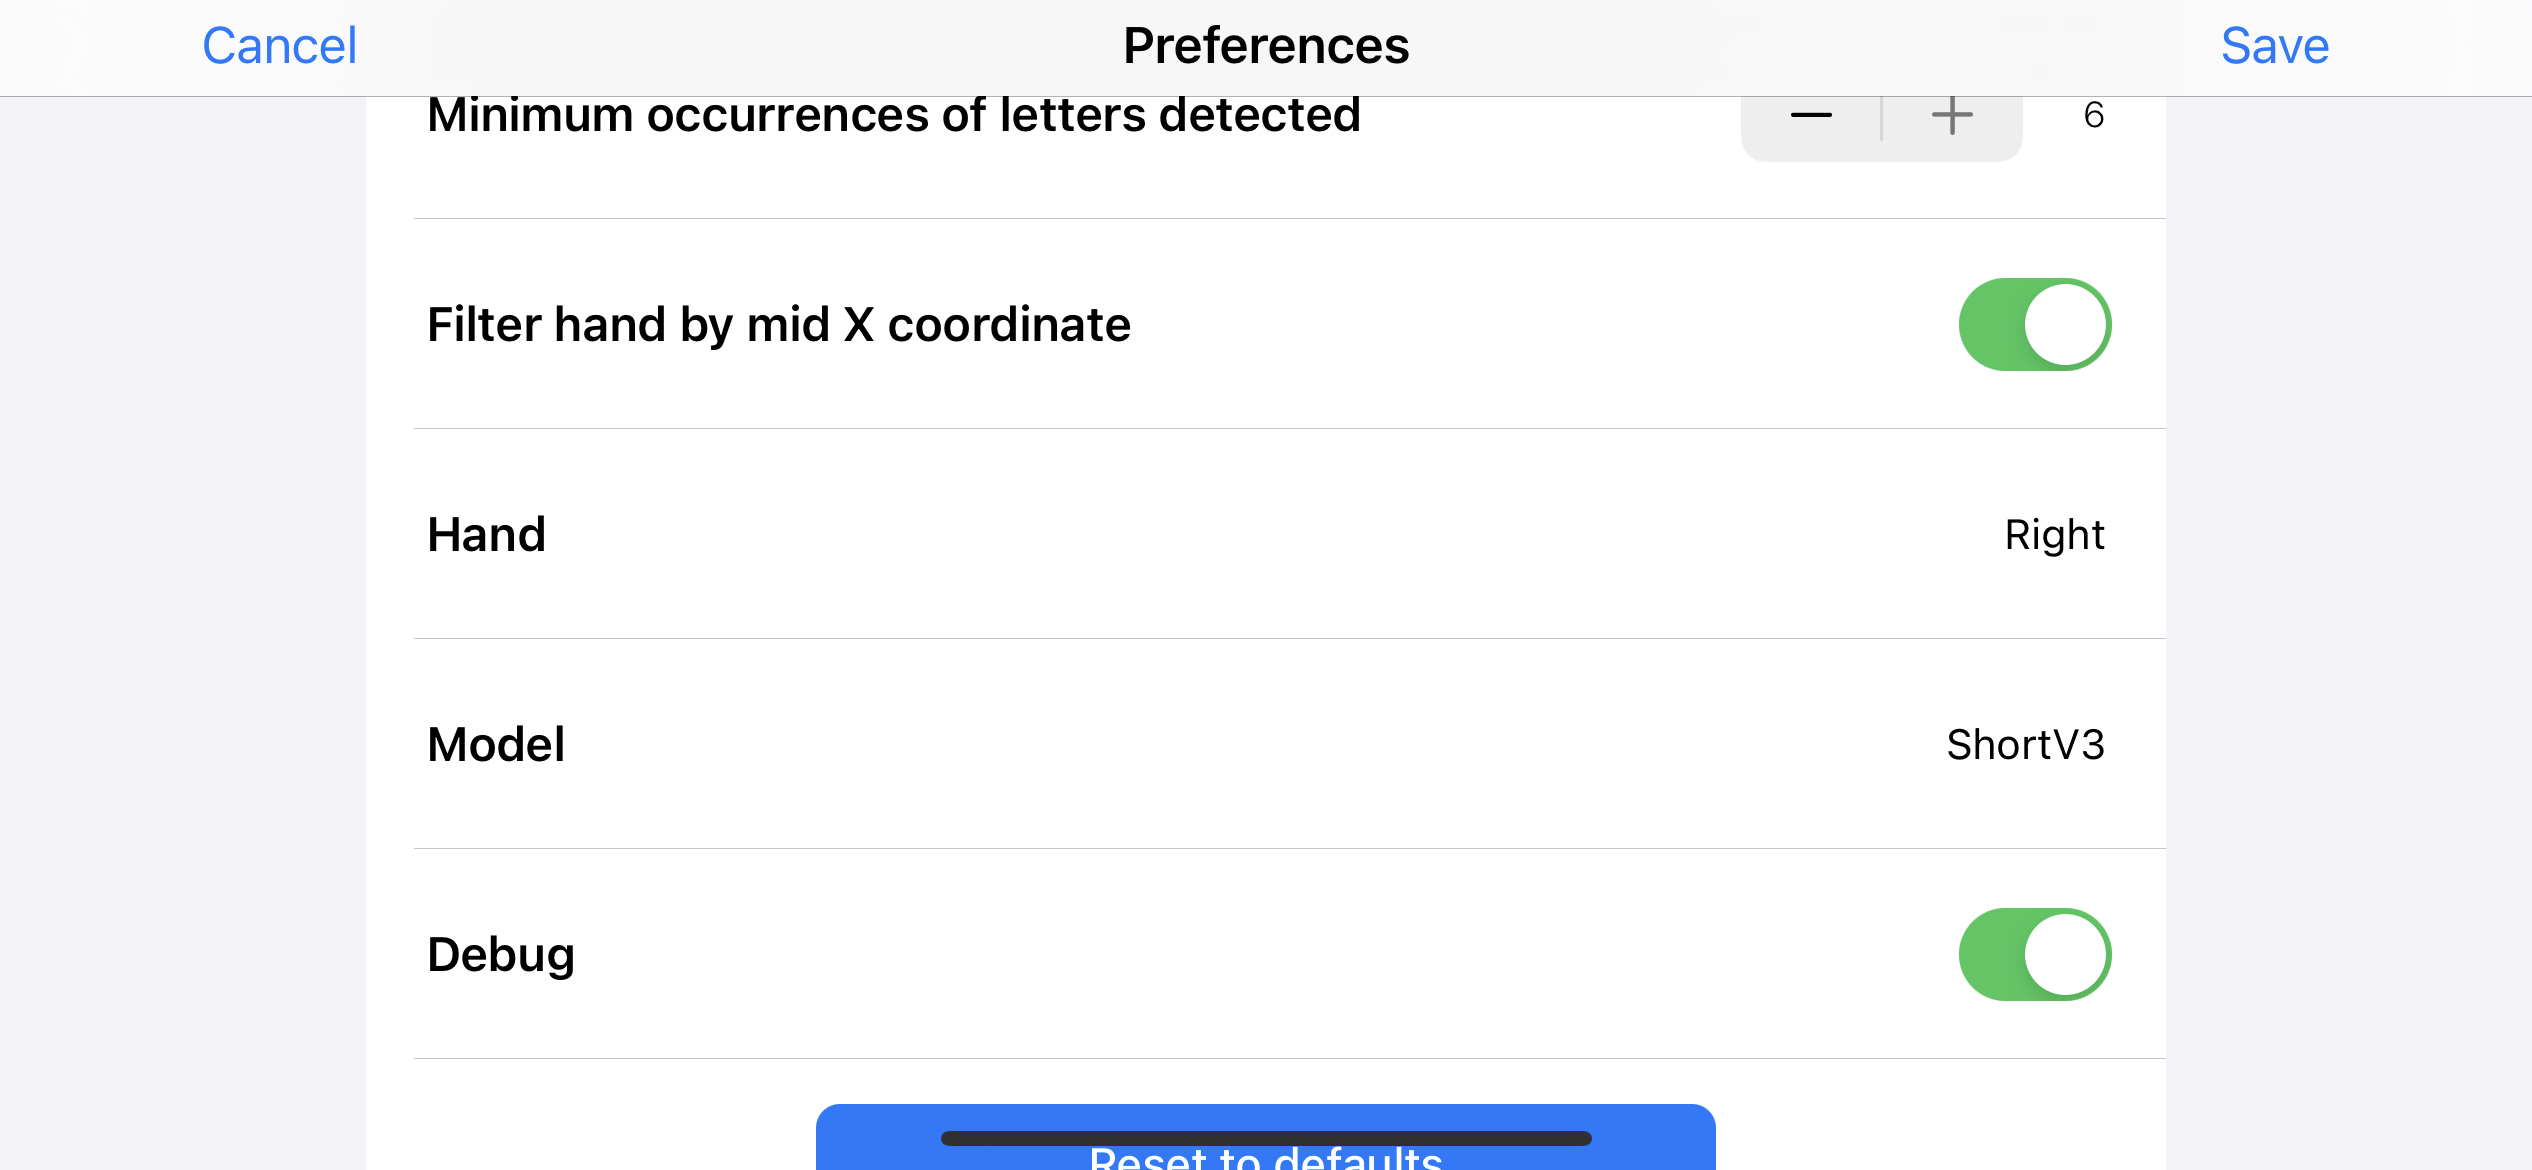
\includegraphics[width=1\textwidth]{images/interpreter/config-scene2.PNG}
\caption{Parámetros de configuración.}
\label{figure29}
\end{figure}

\end{document}